\chapter{System Architektur}
\label{kap:Kapitel03}

\section{Überblick}

Im folgenden wird nun die System Architektur erläutert, welche als Grundlage der Studie diente, um die in 1.2 geschilderte Problemstellung abzubilden und letztendlich zu lösen. 

\subsection{Architektur}
\subsection{Workflow}
\subsection{Entwicklungsprozess}
Abschließend widme ich mich dem Prozess der Entwicklung, aus welchem schließlich die finale Version der Systemarchitektur resultierte. \\
Die Entwicklungszeit betrug ca. 5 Monate und beinhaltete mehrere Iterationen der einzelnen Komponenten bishin zum derzeitigen Stand. Das Konzept sah primär die Entwicklung von drei dedizierten Softwareanwendungen vor, welche aber im Zuge der Iterationen nochmal in kleinere Module aufgeteilt und ausgelagert wurden. Zudem wurden, um den Workflow und das Testen während der Entwicklungsphase zu erleichtern, Anwendungen entwickelt, welche während der Konzeption in der Art nicht vorgesehen waren, aber partiell Bestandteil der Systemarchitektur wurden. \\
So wurde mit zwei separaten Repos gestartet, einerseits für den Learning-Part, welcher anfänglich auch die Smart Contracts umfasste, und andererseits eines für die Mobile-App, welches bereits vor der eigentlichen Konzeption erstellt wurde, um in erster Linie bestehende Crossplattform Frameworks, auf Basis der Kompatibilität und Funktionstüchtigkeit mit Libraries, welche die Kommunikation mit der Blockchain ermöglichen, zu evaluieren. \\
Die Wahl fiel letztendlich auf React-Native, welches zwar nur bis zu einer bestimmten Versionsnummer der Web3.js Library von Ethereum vollends kompatibel ist und nur mit einem kleinen Workaround zum Laufen gebracht werden konnte. 
Jedoch im Vergleich zu anderen Frameworks (z.B. Nativescript) die beste Development-Experience (geringe Lernkurve, gute Dokumentation, CLI) bot und v.a. hinsichtlich der Requirements alle Aufgaben komplett erfüllen konnte, welche die anderen Frameworks in dieser Gänze nicht replizieren konnten. \\
Nachdem die erste rudimentäre Version der Mobile App, welche lediglich eine funktionierende Kommunikation (read/write) mit einem bereits bestehenden Smart-Contract auf einer lokal gehosteten Blockchain bestätigte, erstellt wurde, kam im nächsten Schritt der Learning-Part zum Zuge. \\\\
In Anbetracht der kompletten Implementierung des Ethereum Protokolls in Golang und der Schwierigkeiten mit der Javascript Library Web3.js, v.a. im Bezug auf das deployen der Smart-Contracts, aus einem vorangegangen Projekt, fiel die Wahl für diese Instanz auf Golang. \\
Zuerst wurde der Q-Learning Algorithmus, welcher für das Erlernen des Kaffeetrinkverhalten zuständig ist, implementiert. Die Problematik bestand zum einen darin mit einer neuen Programmiersprache vertraut zu werden und zum anderen den Workflow hinsichtlich der Problemstellung und des daraus resultierenden Zustandsraums vollends abzubilden. Die Umsetzung des Algorithmus in der Programmiersprache ging relativ einfach von der Hand, was jedoch Probleme bereitete war die Simulation des Workflows, um die Algorithmusparameter zu justieren und dessen Tauglichkeit bezüglich das Erlernen des Nutzerverhaltens zu testen.\\\\
Im Anschluss wurde ein erster Smart-Contract erstellt und via dem “go-ethereum” package deployed, woraus das erste Smart-Contract Bidingsfile resultierte, welches für die Kommunikation mit dem Smart Contract vonnöten ist. Da mit jedem neuem Deployement eines Smart Contracts eine neue Smart Contract Addresse und eine neue ABI hervorgeht, welche wiederum beide im Source Code für die Kommunikation mit dem Smart Contract, über alle Instanzen hinweg, die mit einem Smart Contract interagieren wollen, hinterlegt sein müssen, wurde ein kleiner HTTP-Fileserver entwickelt, auf dem diese Informationen gespeichert und gelesen werden können. \\
Bei jedem neuen Deployment wurden daraufhin die Smart-Contract Addresse und die generierte ABI in ein JSON-File gepackt und an den Server geschickt. So konnte während der Entwicklung enorm an Zeit gespart werden, da sich sowohl die Learning-Instanz als auch die App, die benötigten Daten vom Server holten und somit ein ständiges “Hardcodieren” dieser Daten vermieden werden konnte. \\
Aus diesem Grund fand der File-Server auch Einzug in die finale Systemarchitektur, da er als persistente Datenquelle eine enorme Erleichterung nicht nur im Entwicklungsprozess, sondern auch im “Live-System” darstellte. \\
Zudem wird der Fileserver auch für die Verwaltung der Algorithmus-Daten verwendet. Dabei wird bei jedem Worker-Durchlauf (vgl. 3.1.2) für jeden Nutzer ein JSON-File erzeugt, welches folgende Key-Value-Pairs beinhaltet (vgl. Abbildung \ref{img:abb1}): 
\begin{itemize}
	\item qt: die aktuelle Q-Tabelle des Users
	\item ep: der aktuelle Epsilon-Wert
	\item negs: Anzahl der falschen Predictions in der aktuellen Woche
	\item Wk\_negs: Array von negs über alle Wochen hinweg
\end{itemize}


\begin{figure}[th!]
    \centering
    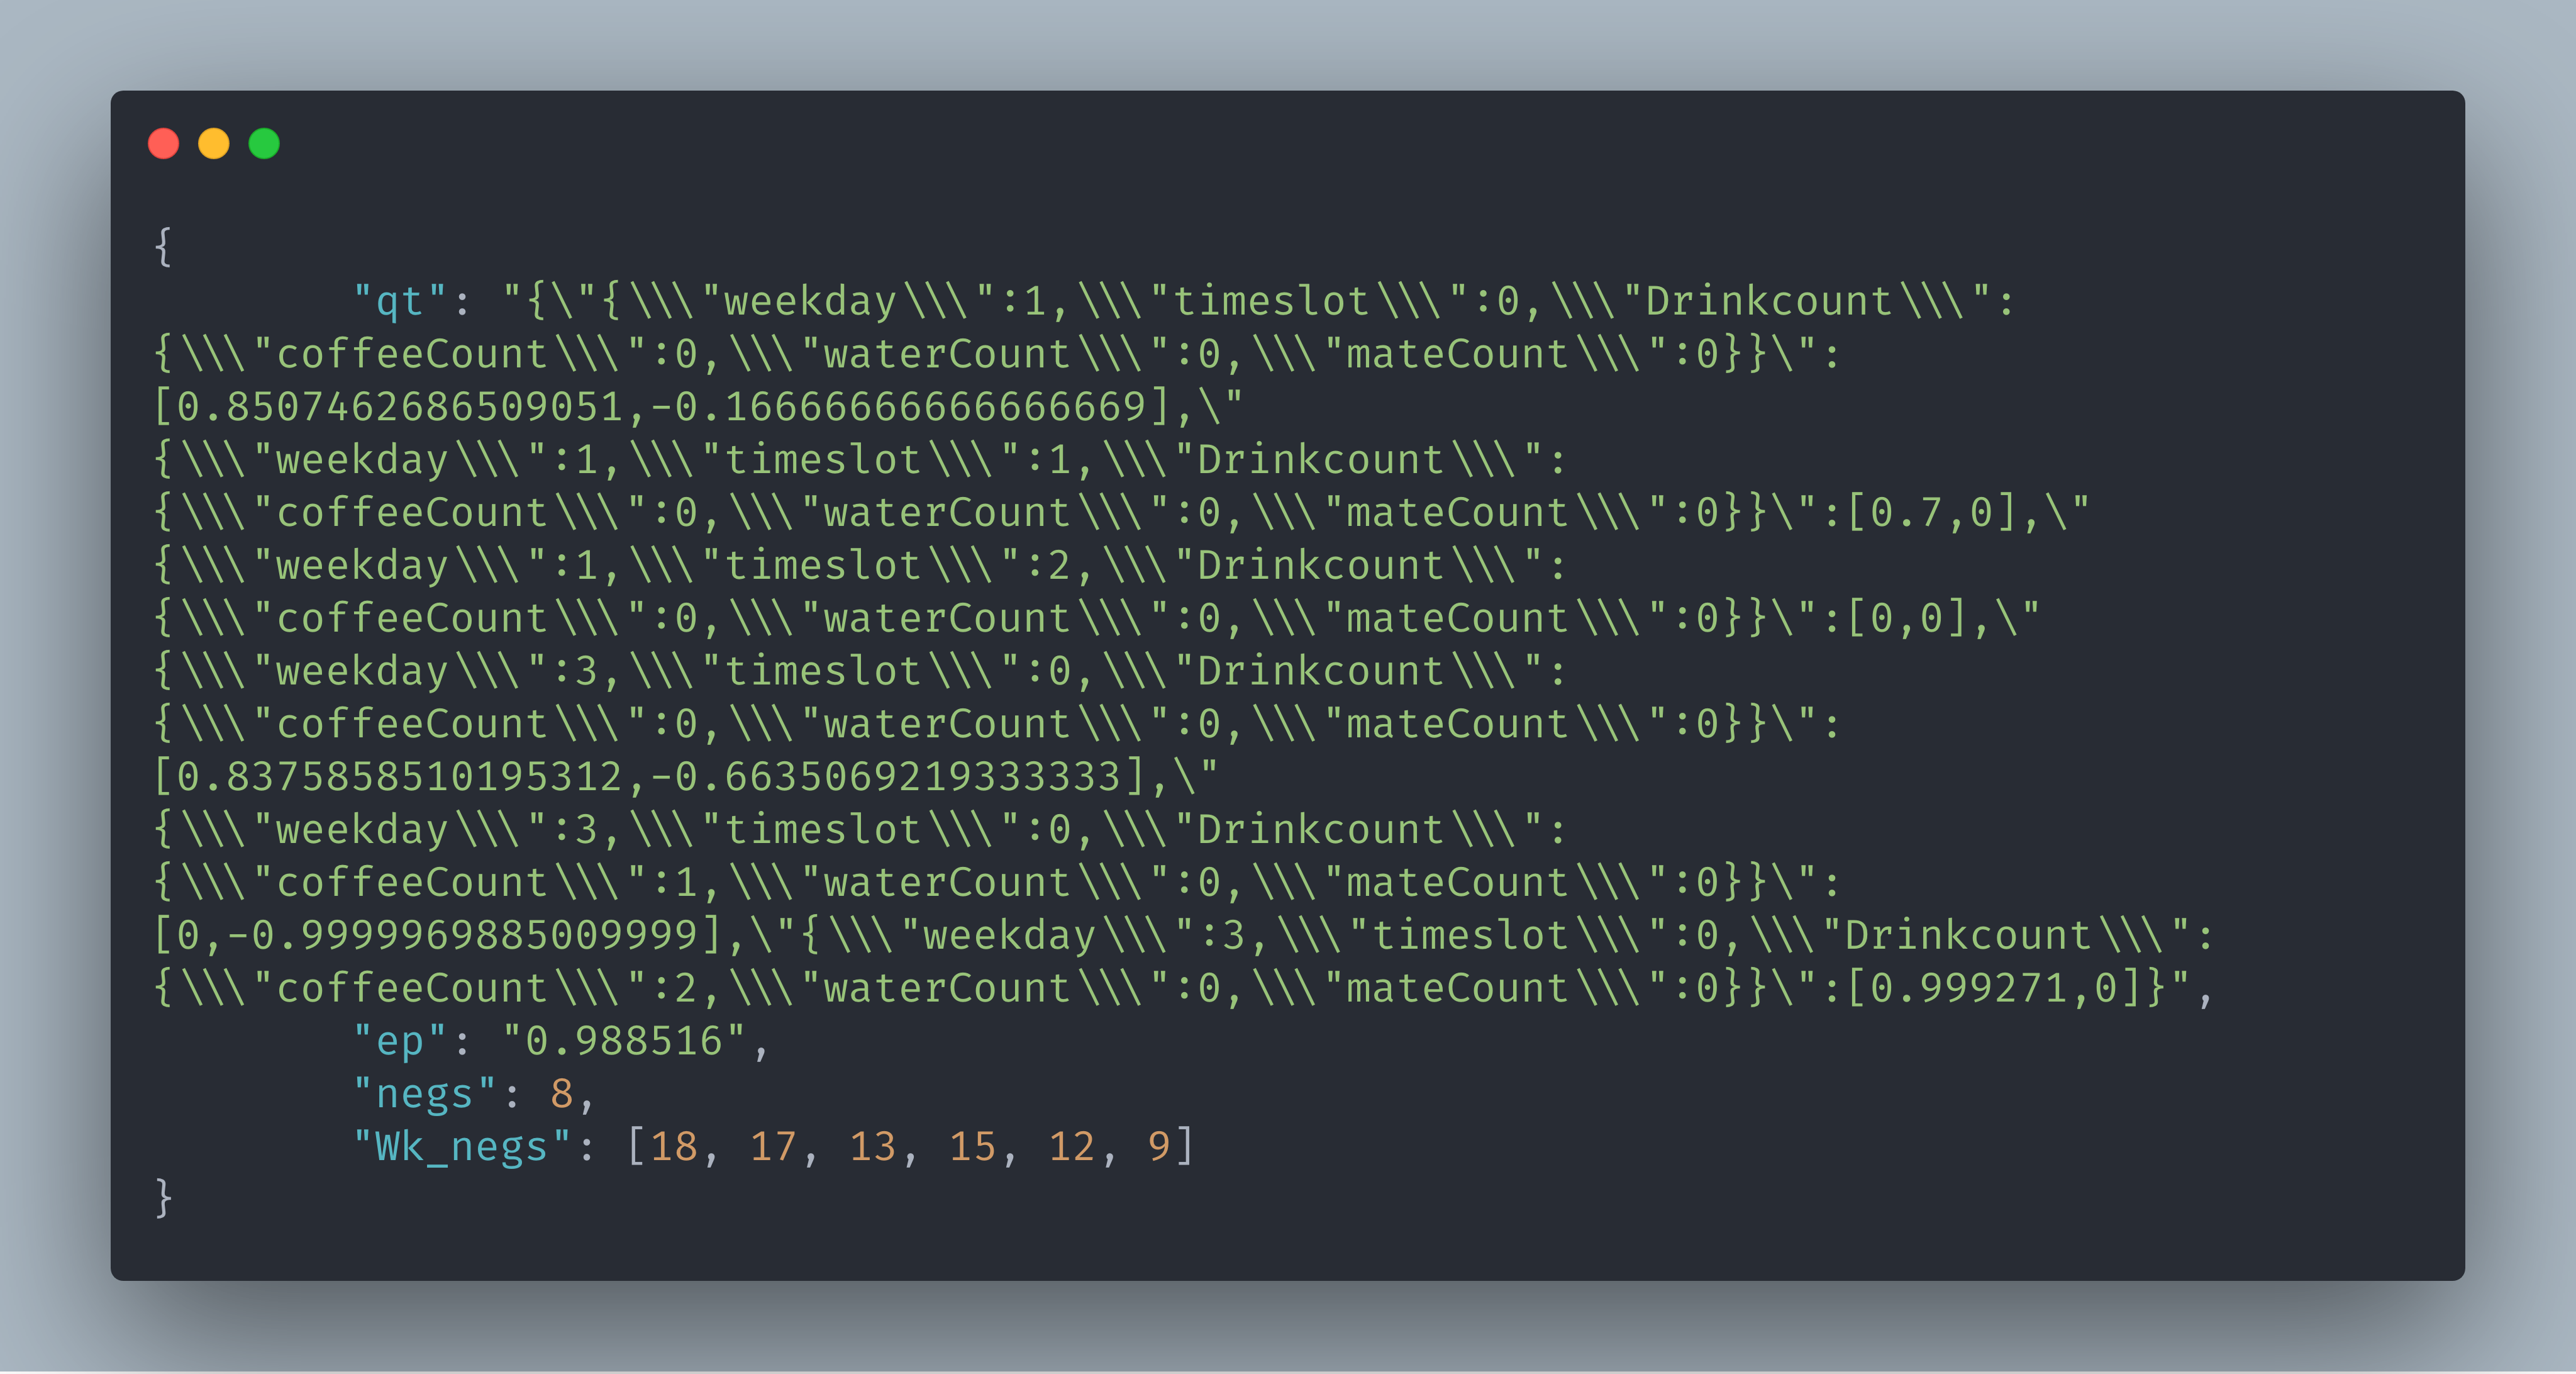
\includegraphics[width=.9\columnwidth]{./Abbildungen/Kapitel_03/usr_json.png}
    \caption{0x6ecbe1db9ef729cbe972c83fb886247691fb6beb-ql.json}
    \label{img:abb1}
\end{figure}

Der Vorteil liegt darin, dass der Learner jederzeit upgedated werden kann ohne die Algorithmusdaten zu verlieren. Denn wird der Learner gestartet, holt sich dieser zuerst die Files vom Server, liest die Daten aus und initialisiert schon im Vorab die Q-Tabelle und das Epsilon eines jeden Users. \\
Sollte der Learner aus unbestimmten Gründen abstürzen, ist durch den eben beschriebenen Algorithmus die Erhaltung des Lernfortschrittes trotzdem sichergestellt.\\\\
Als letztes Modul wurde ein kleiner Node-Server entwickelt, dessen Aufgaben darin bestand die Smart-Contracts zu testen und als primitiver Ersatz für die App zu fungieren. Hierbei erzeugte er in einem festgeleten Intervall (7sek) Events mit einem zufällig generierten Daten (User \& Getränk) auf der Blockchain, um letztendlich die Event-Erkennung (“Watcher”) des “Learners” zu testen. Dabei wurde sowohl für den "Beveragelist-Contract" als auch für den "CoffeeCoin-Contract" eine entsprechende Implementierung angefertigt.
\\In diesen Fällen wurde das Q-Learning-Submodul des Learners gar nicht erst gestartet, da lediglich die Funktionsweise des Watchers getestet werden sollte.\\
Besonders hier zeigte sich die Nützlichkeit des File-Servers, da gerade in der Entwicklungsphase die Smart-Contracts noch häufigen Änderungen unterlagen und dahingehend sehr oft neu deployed werden mussten, was ohne den Fileserver dazu geführt hätte die Smart Contract Daten bei jeder Iteration neu im Sourcecode zu hinterlegen.\\
Nach einer längeren Testphase, in der eine einwandfreie Kommunikation mit den beiden Smart Contracts atestiert werden konnte, wurde mit der eigentlichen Entwicklung der App begonnen, für jene auch Teile der Node-Server Implementierung übernommen werden konnten.\\
Schwierigkeiten traten dabei erst in der Testphase auf, in der festgestellt wurde, dass zu wenig Events vom Learner detektiert werden. Die Ursache dafür lag an der sehr alten Android Version des Tablets, die ist nicht ermöglichte eine direkte Verbindung zum Uni-Netzwerk herzustellen. Dies gelang nur mit einem Workaround, bei dem sich das Tablet mit einem öffentlichen Wlan-Netzwerk verband und sich daraufhin über eine VPN-Verbindung in das Uni-Netzwerk einwählen konnte. \\
Das führte jedoch dazu, dass die Verbindung zum Wlan-Netzwerk in unregelmäßigen Abständen abbrach und dadurch auch zur Blockchain. Da so ein unvorhergesehenes Verhalten wurde in der ersten Implementierung der App nicht vorgesehen war, musste dies in einem Update der App berücksichtigt werden (vgl. 3.4), sodass keine Daten verloren gingen, sollte die Verbindung abbrechen. \\\\
Schlussendlich waren es sechs dedizierte Softwareanwendungen, welche jeweils in eigenen Git-Repositories gehostet werden. 



\section{Blockchain}
\subsection{Beveragelist}
\subsection{ERC-Token}

\section{Q-Learning}
\subsection{Warum Q-Learning?}
\subsection{Modellierung}
\subsection{Lernprozess \& Ablauf}

\section{Mobile App}


